% Document information
\newcommand{\titleinfo}{Zusammenfassung DigitalDesign}
\newcommand{\authorinfo}{Sandro Pedrett}
\newcommand{\version}{1.0}
\newcommand{\versioninfo}{FS22}
% Header
\include{Template/Header}

% Setup Source Code
\lstset{ 
	backgroundcolor=\color{white},   % choose the background color; you must add \usepackage{color} or \usepackage{xcolor}; should come as last argument
	basicstyle=\footnotesize,        % the size of the fonts that are used for the code
	breakatwhitespace=true,         % sets if automatic breaks should only happen at whitespace
	breaklines=true,                 % sets automatic line breaking
	captionpos=b,                    % sets the caption-position to bottom
	commentstyle=\color{ForestGreen},    % comment style
	escapeinside={\%*}{*)},          % if you want to add LaTeX within your code
	extendedchars=true,              % lets you use non-ASCII characters; for 8-bits encodings only, does not work with UTF-8
	frame=single,	                   % adds a frame around the code
	keepspaces=true,                 % keeps spaces in text, useful for keeping indentation of code (possibly needs columns=flexible)
	language=VHDL,                      % the language of the code
	numbersep=5pt,                   % how far the line-numbers are from the code
	rulecolor=\color{black},         % if not set, the frame-color may be changed on line-breaks within not-black text (e.g. comments (green here))
	showspaces=false,                % show spaces everywhere adding particular underscores; it overrides 'showstringspaces'
	showstringspaces=false,          % underline spaces within strings only
	showtabs=false,                  % show tabs within strings adding particular underscores
	stepnumber=2,                    % the step between two line-numbers. If it's 1, each line will be numbered
	tabsize=2,	                   % sets default tabsize to 2 spaces
	title=\lstname,                   % show the filename of files included with \lstinputlisting; also try caption instead of title
	stringstyle=\ttfamily\color{red!50!brown},
	keywordstyle=\color{blue}\bfseries,
}

% 4 A4 Seiten (2 Doppelseiten)


% Document
\begin{document}

\section{Realisierungsformen}
\begin{center}
	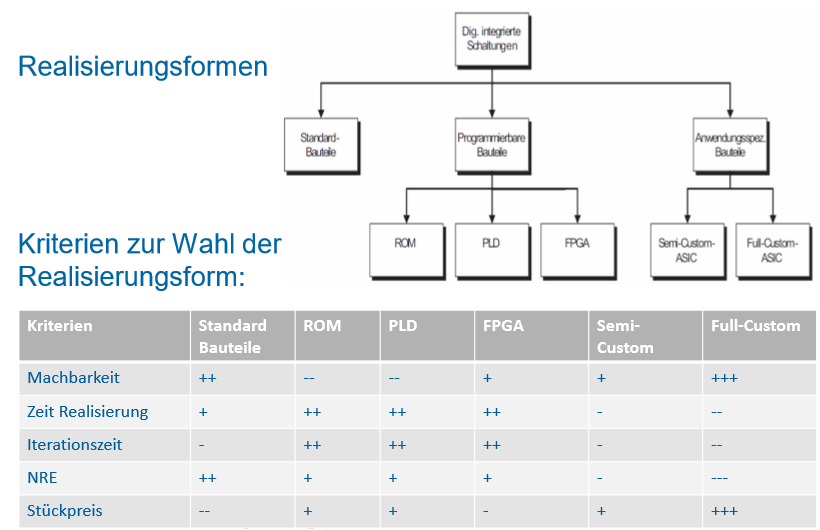
\includegraphics[width=\columnwidth]{Images/realisierungsformen}
\end{center}

\subsection{Standard-Bauelemente}
Komponenten mit fixer Funktion zB USB-Controller, MCU, Gatter etc. Standard-Bauteile werden in grossen Stückzahlen gefertigt. Für komplexere Anwendungen sind jedoch häufig Kombinationen benötigt, was zu einem grösseren PCB führt. Die Kosten sind für NRE sehr gering, können aber auch rasch teuer werden für grössere Stückzahlen. Einsatzgebiet sind Prototypen

\subsection{Programmierbare Bauteile}
\subsubsection{ROM}
Können programmiert werden zB PROM (one time programmable) oder EEPROM (Electrically Eraseable). Die Realisierungszeit ist sehr klein, da einfach der Speicher geändert werden kann. Die Kosten sind relativ gering. Das Einsatzgebiet beschränkt sich jedoch auch Kombinatorischen Schaltungen oder Look-Up-Table (LUT)

\subsubsection{PLD}
Programmable Logic Device verstehet man allgemein programmierbare Bausteine bestehend aus einer AND oder OR Stufe, wovon mindestens eine Stufe programmierbar ist. Für einfach Steueraufgaben sind die Kosten relativ klein. Das Einsatzgebiet wurde jedoch von FPGA fast komplett verdrängt.

\subsection{FPGA}
Field Programmable Gate Array haben ein breites Einsatzgebiet und werden vorallem für das Verarbeiten von grossen Datenmengen zu verarbeiten eingesetzt. Die Kosten sind moderat.

\subsection{ASIC}
Alle Hardware vollständig definierbar und optimiert für Stromverbrauch, Grösse, Funktionalität. Leider sind sehr hohe NRE und langer Designprozess notwendig. Als Anwendung werden diese für alle Extrembereich verwendet.

\subsection{Entwursprozess}
Das y-Modell von DD Gajski beschreibt 3 Sichten mit 5 Hierarchieebenen:
\begin{center}
	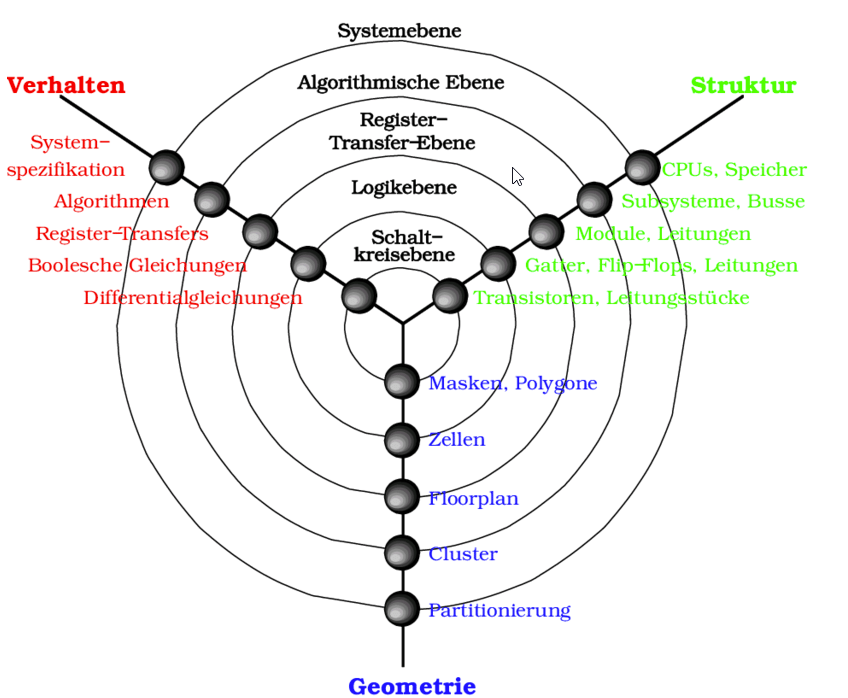
\includegraphics[width=\columnwidth]{Images/y-modell}
\end{center}
 
Der Allgemeine Ablauf fürs das Entwickeln von FPGAs sieht wie folgt aus
\begin{center}
	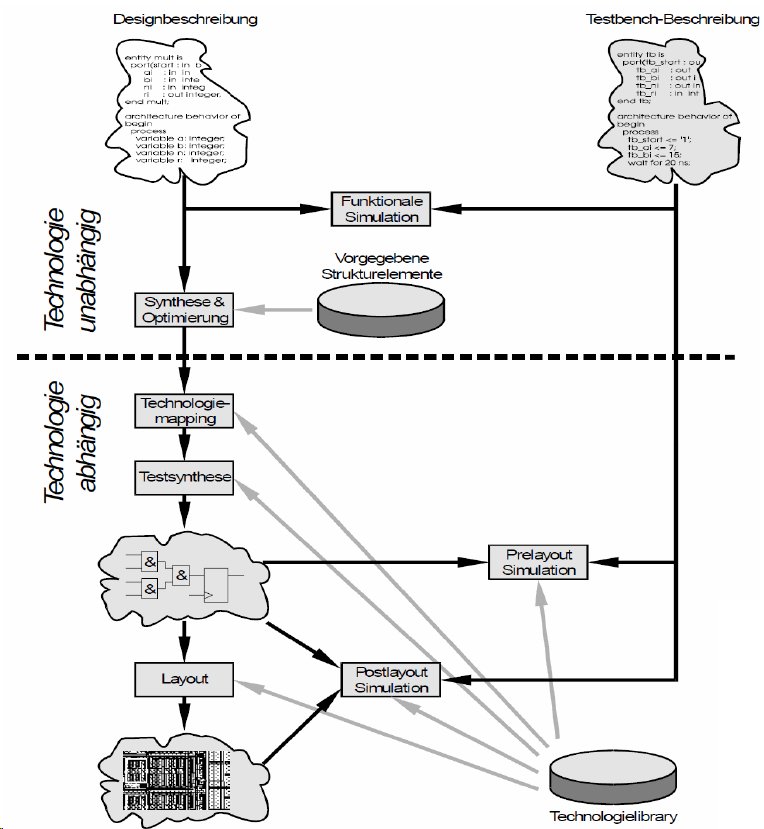
\includegraphics[width=\columnwidth]{Images/ablauf}
\end{center}
Es wird dabei in Frontend (oben), welche Technologie unabhängig ist, und Backend (unten) welche Techonolie abhängig ist unterschieden.\clearpage
\section{VHDL}
Jede VHDL Datei ist durch \textit{Library, Entity, Architecture} definiert. \textbf{Identifier} sind definiert durch:
\begin{itemize}[nosep]
	\item a..zA..Z0..9\_
	\item Start mit Buchstabe
	\item Case insensitive
	\item kein Schlüsselwort
\end{itemize}

\subsection{Library}
Eine Library ist eine Sammlung allgemeiner verwendeten, kompilierten und direkt ausführbaren Code-Blöcken. Dies erlaubt die Wiederverwendung von Code in verschiedenen Projekten.

\begin{lstlisting}
	library ieee; -- ieee standard und work library ohne qualifier verwendbar
	library ams_lib; -- Hersteller spezifische library, Xilinx
	s := ams_lib.tech_data.const1;
	
	-- ohne qualifier nur mit "use" verwendbar
	use ams_lib.tech_data.all;
	s := const1;
\end{lstlisting}


\subsection{Entity}
Entity beschreibt eine Designeinheit als Black-Box. Im Fokus steht die Schnittstelle einer Entwurfseinheit nach aussen, sogennante \textbf{Ports}. Signale dürfen \underline{nicht} in der Port-Liste initialisiert werden.

\begin{lstlisting}
	entity <name> is 
	  port (
	    {<port_name> : <mode> <type>; }
	  );
	end <name>;
\end{lstlisting}
\noindent\textit{mode}
\begin{itemize}[nosep]
	\item \textbf{in}: Eingangsignal darf nur auf rechter Seite stehen
	\item \textbf{out}: Ausgangssignal darf nur auf linker Seite stehen
	\item \textbf{inout}: Bidirektionale Signale, wird mit \textit{std\_logic} verwendet
\end{itemize}

\noindent\textit{type}
\begin{itemize}[nosep]
	\item \textbf{boolean}: \textit{true}, \textit{false}
	\item \textbf{bit}: \textit{'1'}, \textit{'0'}
	\item \textbf{bit\_vector}: eindimensionaler Array von Bits
	\item \textbf{integer}: interne Darstellung von 32 bit Zahlen
\end{itemize}

\subsection{Architecture}
Die architecture beschreibt den inneren Aufbau der Funktionalität, wobei zu einer Entity mehrere Architekturen gehören können. \textbf{Best Practice}: arch\_name ist oft einer der folgenden:
\begin{itemize}[nosep]
	\item \textbf{structural}: Ein und Ausgänge von Komponenten, die in einer Bibliotek abgelegt sind, mit lokalen Signalen verbinden. Netzliste aufbauen
	\item \textbf{behavioral}: Modellierung von Funktionalität
	\item \textbf{tb}: Test Beschreibung, modelliert nur Test-Setup
\end{itemize}

\begin{lstlisting}
	architecture <arch_name> of <entity_name> is
	-- Deklerationen...
	[type_decl]
	[subtype_decl]
	[constant_decl]
	[signal_decl]
	[component_decl]
	begin
	-- Anweisungen...
	end [<arch_name>];
\end{lstlisting}

\subsubsection{Component}
Komponenten (Entities) die innerhalb der Architektur instanziirt werden sollen, müssen deklariert sein.
\begin{lstlisting}
	component <name>
		port(...)
\end{lstlisting}

\subsubsection{Signal}
Interne Signale müssen in der Architecture definiert sein
\begin{lstlisting}
	signal <name> : <type>
\end{lstlisting}

\subsection{Prozesse}
Ein Prozess wird aktiviert, wenn ein Signal in der \textit{sensitivity list} geändert wird. Falls keine sensitivity Liste vorhanden ist, ist der Prozess IMMER aktiv (was nur in TB mit WAIT Statements benötigt wird). Signale werden am ende des Prozess geschrieben. 
\begin{lstlisting}
	[<label>:] process[<sensitivity list>]
	-- Deklerationen...
	[type_decl]
	[subtype_decl]
	[constant_decl]
	[signal_decl]
	[component_decl]
	begin
	-- Sequentielle Anweisungen...
	end process [<label>];
\end{lstlisting}

\subsection{Variable}
Variable sind nur innerhalb von Prozessen gültig. Sie sind nach Zuweisung sofort gültig und müssen nicht auf nächste Prozess Aktivierung warten. Diese sollten immer initialisiert werden, da ansonsten ein D-Latch erstellt wird.
\begin{lstlisting}
	variable <name>: <type> [:= <expression>]
\end{lstlisting}

\subsection{Type}
Aufzählungen werden von links nach rechts codiert zB mit Draycode. Angefangen mit $0$ bis $n$. Diese können in Vivado mit der entsprechende Option festgelegt werden (\textit{fsm\_extraction}).
\begin{lstlisting}
	type <type_name> is ({<identifier> ,?})
\end{lstlisting}

\subsection{Anweisungen}
\subsubsection{If}
If Anweisungen unbedingt mit else abschliessen, ansonsten wird ein Latch erstellt, welcher Hardware-Platz und zusätzliches Timing benötigt.
\begin{lstlisting}
	[<label>:]if <condition> then
		{sequential statements}
	elseif <condition> then
	 	{sequential statements}
 	else
 		{sequential statements}
	end if;
\end{lstlisting}

\subsubsection{case}
Case immer mit \textit{when others} abschliessen, siehe if.
\begin{lstlisting}
	[<label>:]case <condition> is
	{when <choice> => <sequential statement>;}
	when others => <sequential statements>;
	end case;
\end{lstlisting}

\subsubsection{Zuweisung}
Ein \textit{signal} wird der Wert zugewiesen. Bit-Konstante sind mit ' und Vektoren mit \"\ zuzuweisen. Mit concatenate '\&' können signale verbunden werden. 
\begin{lstlisting}
	[<label>:]<signal> <= expression | "1010" | sig1 & "00" | (1=>s(1), 0 => s(0), others => '0') 
\end{lstlisting}
Selektive Zuweisung, sind typisch für kombinatorische Logik mit Verzweigung, müssen alle angegeben werden (mit others). Typisch für Multiplexer.
\begin{lstlisting}
	with <select_sig> select <ausgang_sig> <= 
		{ <eingang_sig> when "00", }
		when others;
\end{lstlisting}
\begin{lstlisting}
	<ausgang_sig> <= { <eingang_sig> when "00" else };
\end{lstlisting}
Diese zwei sind nicht identisch, weil erste parallel ausgeführt, während letztere sequentiell ausgewertet werden, was grossen Einfluss auf Laufzeit hat.

\section{Zustandsmaschiene}
\subsection{UML}
\begin{center}
	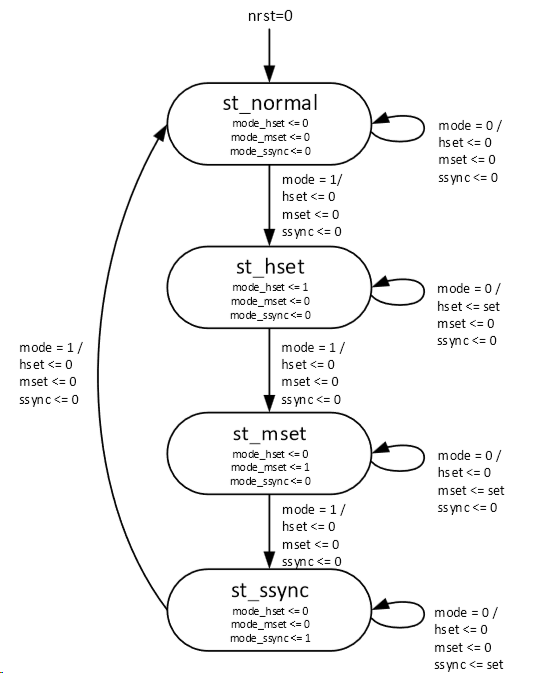
\includegraphics[width=\columnwidth]{Images/zustandsmachine}
\end{center}



\subsection{Sequentielle Systeme - FSM}
Im Gegensatz zu Kombinatorischen Systeme, sind sequentielle Systeme Zustandsbehaftet. Vergangene Verhalten und Eingänge bestimmen momentane Ausgabe, diese sind immer mit einem Takt synchronisiert.
\begin{lstlisting}
library ieee;
	
entity fsm is
port(
	clk : in bit;
	rst : in bit;
	inp : in bit_vector(m-1 downto 0);
	oup : out bit_vector(n-1 downto 0);
);
end;
	
architecture behavioral of fsm is
type state_type is (st_reset, st1, st2, ...); 
signal present_state, next_state: state_type; 

begin
	-- siehe spezifische FSM
end;
\end{lstlisting}
Im folgenden sind 3-Prozesse Strukturen definiert, für 2-Prozesse können Prozess F und G in einem abgehandelt werden, dafür muss aber die sensitivitäts-Liste angepasst werden.


\subsubsection{Mealy Struktur}
Wert der Ausgänge ist von Eingängen und Zuständen Abhängig. Eingänge gehen asynchron durch. Kann zu \underline{Timing Problemen} führen!

\begin{center}
	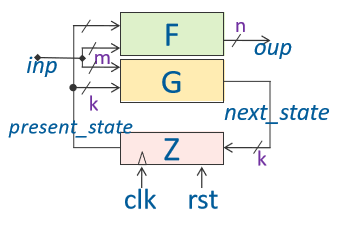
\includegraphics[width=0.4\columnwidth]{Images/mealy_fsm} 
\end{center}
\begin{lstlisting}
	-- Process F
	output_logic: process(inp, present_state)
	begin
	-- default
	oup <= "00";
	
	if (present_state = st1 and inp = "10") then
	oup <= "10";
	-- alle States inkl else
	end if;
	end process;
	
	-- Process G
	next_state_logic: process(inp, present_state)
	begin
	-- default
	next_state <= st_reset;
	
	case present_state is -- folgezustand
	when st1 =>
	if (inp = "10") then
	next_state <= st2;
	end if;
	when ..
	when others => null
	end case;
	end process;
	
	-- Process Z
	state_register: process (clk)
	begin
	if (rising_edge(clk)) then
	if (rst = '1') then
	present_state <= st_reset;
	else 
	present_state <= next_state;
	end if
	end process;
\end{lstlisting}


\subsubsection{Moore Struktur}
Wert der Ausgänge ist nur vom aktuellen Zustand des Systems abhängig.

\begin{center}
	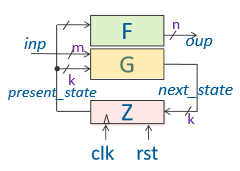
\includegraphics[width=0.4\columnwidth]{Images/moor_fsm}
\end{center}
\begin{lstlisting}
	-- Process F
	output_logic: process(present_state)
	begin
	-- default
	oup <= "00";
	
	if (present_state = st1) then
	oup <= "10";
	-- alle States inkl else
	end if;
	end process;
	
	-- Process G
	next_state_logic: process(inp, present_state)
	begin
	-- ..
	end process;
	
	-- Process Z
	state_register: process (clk)
	begin
	-- ..
	end process;
\end{lstlisting}

\subsubsection{Medwedjew Struktur}
Spezialfall des Moore-Systems: Ausgänge entsprechen dem Zustandsvektor. zB für Zähler.

\begin{center}
	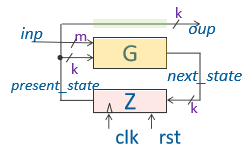
\includegraphics[width=0.4\columnwidth]{Images/med_fsm}
\end{center}
\begin{lstlisting}
	-- Process G
	next_state_logic: process(inp, present_state)
	begin
	-- ..
	end process;
	
	-- Process Z
	state_register: process (clk)
	begin
	-- ..
	end process;
	
	oup <= present_state
\end{lstlisting}


\section{Simulation}

\subsection{Delay-Modell}
Das Transport-Modell (1) verzögert in jedem Fall um die mit \textit{after} definierte Zeit.\\
Das Inertial-Modell (2) muss länger als die mit \textit{after} definierte Zeit sein, ansonsten wird dieser verschluckt.
\begin{lstlisting}
	-- (1)
y <= transport a or b after 10 ns;
	-- (2), auch inertial
y <= a or b after 10 ns;
\end{lstlisting}

\subsection{Testbanche}
\begin{lstlisting}
library ieee;

entity glue_logic_tb is
-- meist leer
end;

architecture tb of glue_logic_tb is
	component glue_logic
		port(in0 : in  bit);
	end component glue_logic;
	
	for all : glue_logic use entity work.glue_logic(behavioral);
	
	constant SIM_CYC : time := 100 ns;
begin

dut : component glue_logic
	port map(in0 => tb_in0);

clock_p : process
begin
	clk <= '1'; wait for (SIM_CYC/2);
	clk <= '0'; wait for (SIM_CYC/2);
end process;
s0 <= '0', 
      '1' after 20ns,
      '0' after 10ns,
      '1' after 60ns;
end tb;

\end{lstlisting}

\section{Beispiele}
\subsection{Pull-Up Treiber}
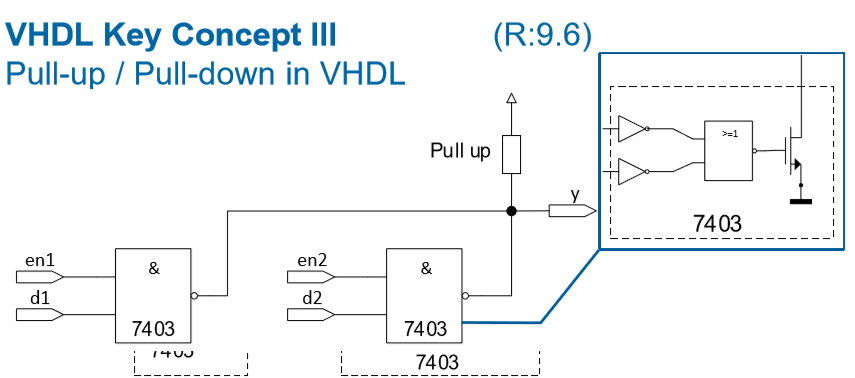
\includegraphics[width=\columnwidth]{Images/pullup}
\begin{lstlisting}
pull_up : y <= 'H';

p1 : process(en1, d1)
	begin
		y <= 'Z';
		if en1 = '1' and d1 = '1' then
			y <= '0';
		end if;
	end process;
	
p2 : process (en2, d2)
	begin
		y <= 'Z'
		if en2 = '1' and d2 = '1' then
			y <= '0';
		end if;
	end process;
\end{lstlisting}

\subsection{Bidirektionaler Bus}
\begin{center}
	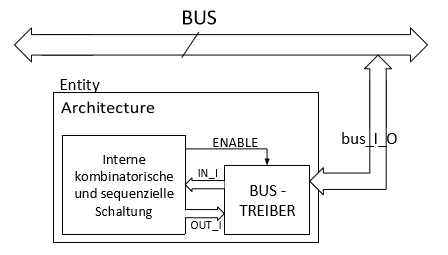
\includegraphics[width=0.8\columnwidth]{Images/bus}
\end{center}
\begin{lstlisting}
bus_write_p : process(enable, out_i)
	begin
		if enable = '1' then
			bus_i_o <= out_i;
		else
			bus_i_o <= (others => 'Z');
		end if;
	end process;
	
	bus_read : in_i <= bus_i_o; -- paralleler lesevorgang
\end{lstlisting}


\subsection{Latch}
\begin{center}
	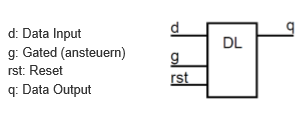
\includegraphics[width=0.5\columnwidth]{Images/latch}
\end{center}
Um ein Speicherverhalten zu simulieren, kann ein Latch verwendet werden. 
\begin{lstlisting}
process(rst, d, g)
begin
	if (rst = '1') then
		q <= '0' 
	elsif (g = '0') then
		q <= d
	else 
		null
end
\end{lstlisting}
\section{Library}
\subsection{IEEE 1164}
9-wertige Logiksystem von IEEE von std\_\textit{u}logic
\begin{center}
	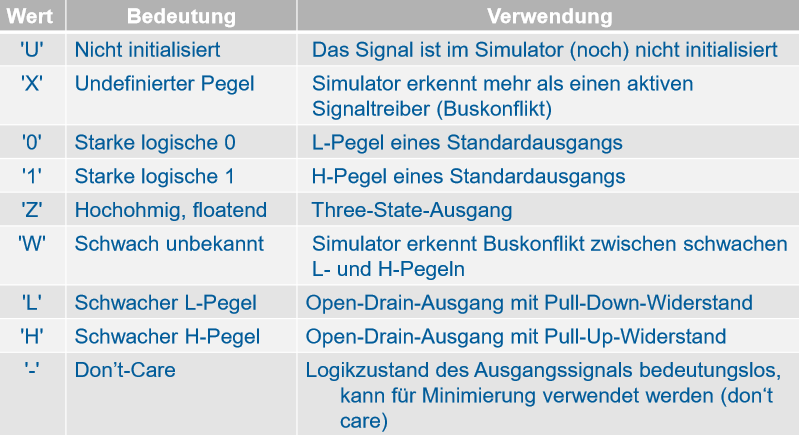
\includegraphics[width=\columnwidth]{Images/ieee_typen}
\end{center}
\textbf{std\_ulogic} akzeptiert nur einen Treiber pro Signal. Compiler erkennt Signalkonflikt und bricht mit Fehlermeldung ab.\\~\\
\textbf{std\_logic} akzeptiert mehrere Treiber pro Signal. Deshalb wird dieser Datentype für bidirektionale Busse eingesetzt. Entscheid, welcher Treiber sich durchsetzt, fällt der Simulator.
\begin{center}
	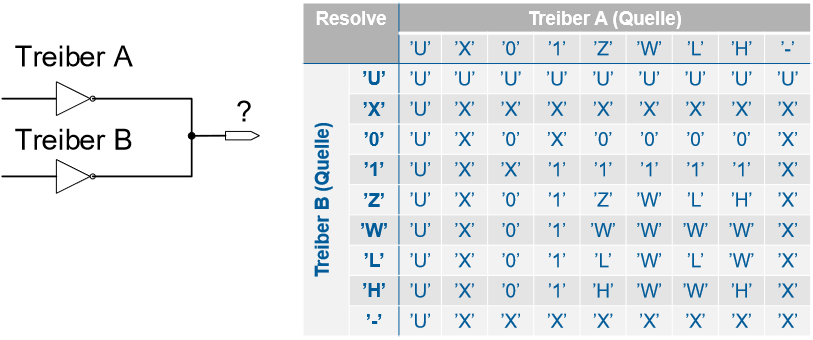
\includegraphics[width=\columnwidth]{Images/ieee_typen1}
\end{center}

\noindent\textbf{Type Cast}
\begin{center}
	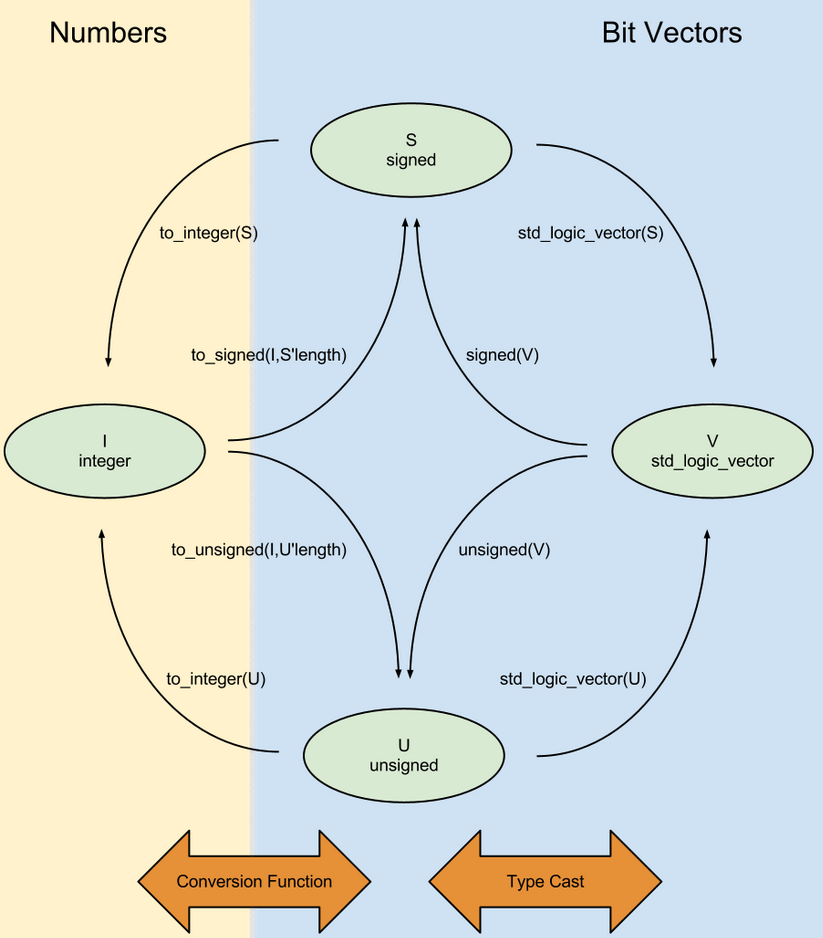
\includegraphics[width=0.8\columnwidth]{Images/type_cast}
\end{center}

\noindent\textbf{Operatoren}
\begin{center}
	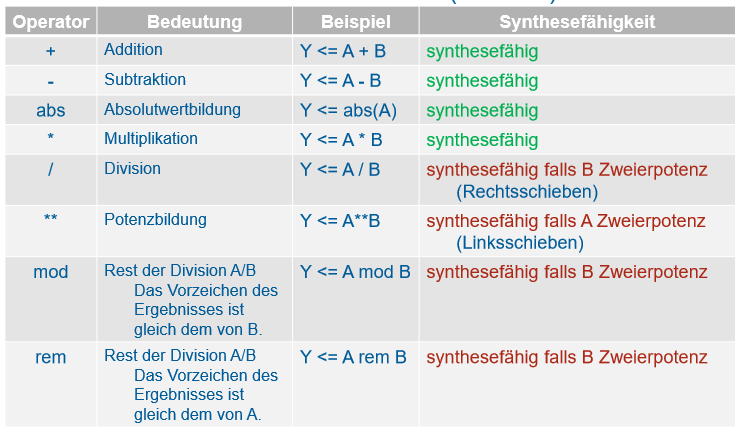
\includegraphics[width=\columnwidth]{Images/type_operator}
\end{center}
\clearpage


\end{document}